\documentclass[11pt,a4paper]{article}

%%% PACKAGES AND FORMATTING

%% MATH PACKAGES AND SYMBOLS

% Math Packages
\usepackage{amsmath}
\usepackage{amsfonts}
\usepackage{amssymb}
\usepackage{siunitx}
\usepackage{bm} % bold fonts for math symbols
\usepackage{mathtools}

% Argmin Operator
\DeclareMathOperator*{\argmin}{argmin} % no space, limits underneath in displays
% Aspect Ratio Symbol
\usepackage{ar}


%% FORMATTING

% Set Margin
\usepackage[left=2cm,right=2cm,top=1.5cm,bottom=1.5cm]{geometry}

% Remove Auto-Indent
\setlength{\parindent}{0pt}

% Tabu Table Package
\usepackage{tabu}

% Chapter Header in One Line
\usepackage{titlesec}
\titleformat{\chapter}[hang] 
{\normalfont\huge\bfseries}{\chaptertitlename\ \thechapter}{1em}{}


%% GRAPHICS AND CAPTIONS

% Graphics Package
\usepackage{graphicx}

% Caption Package
\usepackage{caption}
\usepackage{subcaption}

% Item Placement Package
\usepackage{float}

%% HYPERLINK PAGES

\usepackage{hyperref}

	
\begin{document}

\begin{titlepage} %% TITLE PAGE

\rule{\textwidth}{1.6pt}\vspace*{-\baselineskip}\vspace*{2pt}
\rule{\textwidth}{0.4pt}\\[\baselineskip]
\vspace*{-1cm}
\begin{center}
\huge{\bf Brief of an Euler-Bernoulli Beam Solver}
\end{center}
\rule{\textwidth}{0.4pt}\vspace*{-\baselineskip}\vspace*{3.2pt}
\rule{\textwidth}{1.6pt}\\[\baselineskip]

\vspace{8cm}

% Information
\centering{
	\begin{tabular}{rl}
	\\
	{\bf    Department:} & {Department of Aeronautics}   
	\\
	{\bf Student:} & {Wee Zhao, Chua Khoo}
	\\
	{\bf CID:} & {01117650}   
	\\
	{\bf Date:} & {\today}  
	\end{tabular}
}

\vspace*{\fill}

\end{titlepage}

\pagenumbering{roman}

% Format Page Numbering
\newpage
\setcounter{page}{1}
\pagenumbering{arabic}

\section{Formalism}
This document acts as a brief to a set of MATLAB scripts which solves an Euler-Bernoulli beam. The beam equations are as seen in the Introduction to Structural Analysis course, with the notes included for reference. Only the crux of the solution algorithm are presented. For an in-depth understanding of the implementation details refer to the documentations in the script.
\subsection{Sign Convention}
Over the span of a beam, we adopt a sign convention where the beam extends from left to right, and a \textit{virtual cut} is made on the right facing face. A positive shear, $F(z)$, is defined to act upwards, while a positive moment, $M(z)$, is defined to act clockwise. A vertical force loading is defined positively acting upwards, with a positive point moment load acting clockwise. See Figure \ref{fig:sign_convention} for reference.
\begin{figure}[H]
\centering
	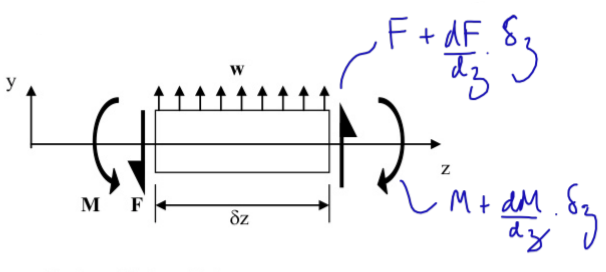
\includegraphics[scale=0.8]{sign_convention.png}
	\caption{Sign convention as defined in the positive sense.}
	\label{fig:sign_convention}
\end{figure}
\subsection{Beam Configuration}
Here, we clarify the beam configurations supported by the scripts. For every beam configuration, there is an implicit assumption that there is at least one lateral force present, fixing the beam laterally. For both ends of a beam, there are options for a free ended beam, a simple support and a cantilever support. Between two ends of a beam, there can exist arbitrary number of simple supports. On the other hand, for load configurations, the scripts support a distributed load across the span of the beam. Arbitrary number of point force and moment loads are supported as well. A combination of all these support and loading can be handled by the solver. The scripts allow for a varied second moment of inertia, $I(z)$, with a varied height, $y(z)$, across the span of the beam.
\newpage
\section{Solution Algorithm}
The behaviour of an Euler-Bernoulli beam is governed by a fourth-order differential equation
\begin{equation*}
	\left( E \, I(z) \, v^{''}(z) \right)^{''} = w(z).
\end{equation*}
Over the span of a beam, the internal shear and bending moments are determined by the forces and moments exerted over the span of the whole beam. Discontinuities in the internal shear and bending moments over the span of a beam arises from two sources: i) the force and moment exerted by a simple/cantilever support or ii) the forcing exerted by a point vertical load/moment. The main strategy to automate the solution process is to split a beam down into sections at points where discontinuities in shear or bending moment appears. The beam is integrated in the $z$ direction as usual, but to identify the reaction forces contributed from supports and the resultant deflections, a system of linear equations is formulated based on the boundary conditions at the ends of each beam section and the vertical force equilibrium condition.
\subsection{Section of an Euler-Bernoulli Beam}
For a section of the beam (from $z_i$ to $z_j$) permitting a continuous solution in the internal shear and bending moments, the equation reduces to a fourth order differential equation with four boundary conditions required to solve for the integration constants.
\begin{align}
	 \left( E \, I(z) \, v^{''}(z) \right)^{''} & = w(z)\\
	-F(z) = \left( E \, I(z) \, v^{''}(z) \right)^{'} & = \int_{z_i}^{z_j} w(z) \, dz + A \\
	-M(z) = E \, I(z) \, v^{''}(z) & = \int \int_{z_i}^{z_j} w(z) \, d^2z + Az + B \\
	v^{'}(z) & = \int_{z_i}^{z_j} \frac{1}{E \, I(z)} \left[ \int \int_{z_i}^{z_j} w(z) \, d^2z + Az + B \right] dz  + C \\
	v(z) & = \int \int_{z_i}^{z_j} \frac{1}{E \, I(z)} \left[ \int \int_{z_i}^{z_j} w(z) \, d^2z + Az + B \right] d^2 z  + Cz + D
\end{align}
The implementation solves the differential equation by using a rectangular numerical integration, with $A$, $B$, $C$, $D$ treated as a set of unknown scaling constants for $F(z)$, $M(z)$, $v^{'}(z)$ and $v(z)$. The unknowns will be solved by forming a system of linear equations coming from the boundary conditions required at both ends of a beam section. Each beam section will lead to $4$ linear equations that is required to be solved. The boundary conditions for a beam section is derived from the specified load and support configuration.
\subsection{Boundary Conditions: $z = 0$}
The boundary conditions are
\subsubsection*{Free-ended Beam}
\begin{align}
	F = 0 \\
	M = 0
\end{align}
\subsubsection*{Cantilever Support}
\begin{align}
	v^{'} = 0 \\
	v = 0
\end{align}
\subsubsection*{Simple Support}
\begin{align}
	M = 0 \\
	v = 0
\end{align}
\subsubsection*{Applied Point Load (Force and Moment)}
\begin{align}
	F = -F_{\text{applied}} \\
	M = -M_{\text{applied}}
\end{align}
\subsection{Boundary Conditions: $0 < z < L$}
For a beam with discontinuous solutions in shear force and bending moment, we make a distinction between properties of the left beam segment with the notation $(\cdot)_{L}$ and the right beam section with the notation $(\cdot)_{R}$.\\
\\
The boundary conditions are
\subsubsection*{Simple Support}
\begin{align}
	M_{L} &= M_{R} \\
	v_{L}^{'} &= v_{R}^{'} \\
	v_{L} &= 0 \\
	v_{R} &= 0
\end{align}
\subsubsection*{Applied Point Load (Force and Moment)}
\begin{align}
	F_{L} - F_{R} &= F_{\text{applied}} \\
	M_{L} - M_{R} &= M_{\text{applied}}	\\
	v_{L}^{'} &= v_{R}^{'} \\
	v_{L} &= v_{R}
\end{align}
\subsection{Boundary Conditions: $z = L$}
The boundary conditions are
\subsubsection*{Free-ended Beam}
\begin{align}
	F = 0 \\
	M = 0
\end{align}
\subsubsection*{Cantilever Support}
\begin{align}
	v^{'} = 0 \\
	v = 0
\end{align}
\subsubsection*{Simple Support}
\begin{align}
	M = 0 \\
	v = 0
\end{align}
\subsubsection*{Applied Point Load (Force and Moment)}
\begin{align}
	F &= F_{\text{applied}} \\
	M &= -M_{\text{applied}}
\end{align}
\subsection{Solving the Linear Equations}
By obeying the boundary conditions stated above, every beam section introduces 4 linear equations to be solved (2 at each ends of a section), leading to a full rank matrix, with the $A$, $B$, $C$ and $D$'s of each section from eq.(2) - eq.(5) being the unknown coefficients. Solving the equation and adding up the unknown coefficients, we regain the correct shear, bending moment, gradient and vertical displacement of the beam.
\subsection{Reaction Forces and Moments}
The boundary conditions for a simple support does not require a specification on the shear force. For a cantilever support, there is also no requirement for the shear and moments from the boundary conditions. The reaction forces and reaction moments of these support are determined after the unknown coefficients are solved by a simple local equilibrium analysis once the internal shear and bending moments of the left and right section of the beam is solved.
\section{Code Interface}
Here, we describe the manner an user specifies a beam and go through the steps to interface with the code and how to interpret the solution.
\subsection{Beam Description}
An user starts off by first describing the beam in the script \textit{beam\_config.m}, providing information on the material, geometrical properties and the beam configuration (loads and supports of the beam).\\
\\
The beam configuration is encoded in a numerical matrix format called \textit{bound}, where each row is made up of 4 columns representing the position, boundary type, force applied and moments applied respectively. The user is expected to define this matrix. Position is in units of metres, while the force and moments applied is in Newtons and Newton metres. For the boundary type, a simple support is represented as the numerical value (1), a cantilever support (2), while an applied force/moment (3). When the boundary type is (3), the user is expected to also specify the applied force in the 3rd column and the applied moment in the 4th. A boundary type of (0) represents a free ended beam at $z = 0$ or $z = L$.\\
\\
By running the script, a \textit{.mat} workspace is saved with the name of \textit{beam.config}, containing a \textit{beam} struct. \textit{beam} contains all the information to solve the beam configuration.
\subsection{Beam Solution}
To solve for a beam, the user loads the beam configuration defined in \textit{beam\_config.m} to \textit{beam\_solver.m} and runs it. The beam is solved and the results of bending moment, shear, gradients and displacements are defined in the \textit{res} struct.\\
\\
Internally, stress analysis is carried out and it will inform the user if the loading have exceeded the yield stress of the beam. To identify the reaction forces from the support points, the user inspects the \textit{bound} matrix in the \textit{beam} struct, where the 3rd and 4th column of the corresponding support now displays the reaction forces and moments.
\end{document}